\begin{abstract}
Most bias audits of audio language models use synthetic speech and assume a synthetic voice is treated like a real one. We test this with the speaker and the words held fixed. From 40 LibriSpeech readers we take 200 real utterances and make three matched versions of each: a zero-shot clone of the same speaker, a 6 kbps neural-codec re-encoding of the real recording, and a stock synthetic voice. Three models transcribe, grade, answer questions about, reply to, and judge the provenance of every clip. Gemini 3.6 Flash grades the clone within 0.005 points of the real recording on a 10-point scale (95\% interval $\pm0.16$, $n=200$), with equal word error rate and comprehension. Gemini 3.1 Pro ($+0.35$, interval $-0.90$ to $+1.46$, $n=60$) and Voxtral-Mini-3B ($-0.18$, interval $-0.40$ to $+0.05$, $n=40$) show no significant clone effect either. The codec re-encoding, however, costs 0.31 points on Flash ($p = 3.5\times10^{-4}$), the only effect of 49 that survives correction. Asked directly, the models cannot tell real from clone (balanced accuracy 0.555, 0.54, 0.50); the Gemini models call 74.5\% and 90\% of real recordings synthetic, and Voxtral calls every clip real. Earlier unmatched comparisons reported synthetic-versus-real gaps in both directions, some larger than 12 points; with speaker and words matched, the Gemini gap is zero. Synthetic stimuli are valid for auditing these models if both arms share the same compression.
\end{abstract}

\section{Introduction}
\label{sec:intro}

A voice agent hears a caller and then transcribes, grades, answers, or replies. More and more often the caller is not a person speaking directly. People who use augmentative communication devices speak through text-to-speech, voice-banking users speak through a clone of the voice they lost, agents call other agents, and in a 2026 honeypot study of unwanted calls at least 27\% opened with a machine voice, about half of them with fresh audio that a detector labels synthetic \citep{a2609_11137}. Deployed audio models therefore hear synthetic voices every day, and they are expected to treat them the same as real ones.

Research on these models makes the same assumption. Bias audits need many voices saying the same words, and text-to-speech is the cheap way to get them. Of 21 recent audio-LLM bias and fairness audits we reviewed, 16 use only synthetic stimuli \citep{a2510_02352,a2602_01030,a2511_06592,a2603_16941}. At least three of them name the assumption as an untested limitation \citep{a2509_22061,a2604_14548,a2602_04796}.

Earlier work has compared synthetic and real speech, but without matching. Audio MultiChallenge re-rendered its human turns with a stock TTS voice, and text-output models scored 7.5\% higher (relative) on the synthetic version while audio-output models scored 2.5\% lower \citep{a2512_14865}. MedMosaic reports that Gemini models score 1.4 to 3.3 points higher on an ElevenLabs subset while most open-weight models drop, four of them by more than 12 points \citep{a2605_00969}. VoiceBench reads the same questions with a TTS voice and with crowd-recorded speakers, and reports that every model does better on the synthetic version \citep{a2410_17196}. A separate line of work asks audio models directly whether speech is synthetic and finds answers at or below chance \citep{a2505_11079,a2512_10652}.

\textbf{The gap.} In every one of these comparisons the synthetic and real arms contain different speakers, and often different items and recording conditions, so the measured difference mixes provenance with content, voice identity and audio quality. The explicit-detection studies measure only what the model says, not what it does. Nobody has held the speaker and the words fixed, separated provenance from codec artifacts, and measured behaviour and self-report on the same clips.

We built that comparison (Figure~\ref{fig:schematic}). Each real utterance gets three matched versions: CLONE (same speaker, same words, zero-shot cloned), RESYNTH (the real recording through a 6 kbps neural codec), and STOCK (a default synthetic voice, same words). CLONE minus REAL measures the provenance effect, RESYNTH minus REAL the effect of codec artifacts alone, and STOCK minus REAL the effect of a synthetic voice that is not this speaker. Our contributions are:

\begin{enumerate}
\item \textbf{A matched provenance benchmark.} 200 LibriSpeech items from 40 readers, each in four arms (850 clips including a clone-stability set), loudness-matched and hashed before any model call, with a codec control and a stock-voice control (Section~\ref{sec:setup}).
\item \textbf{The clone has no effect on behaviour.} Gemini 3.6 Flash grades the clone $+0.005$ points from the real recording (interval $-0.16$ to $+0.16$, $n=200$), with equal word error rate (2.7\% vs 2.9\%), comprehension (99.5\% on both) and assistant replies. Gemini 3.1 Pro agrees within a wider interval (Section~\ref{sec:results-clone}).
\item \textbf{The codec does have an effect.} The re-encoded real recording is graded 0.31 points lower ($p = 3.5\times10^{-4}$, $d_z=-0.25$), the only effect in 49 tests that survives correction. This also shows the design has enough power to detect a third-of-a-point shift (Section~\ref{sec:results-codec}).
\item \textbf{Self-report is near chance and biased.} Real-versus-clone balanced accuracy is 0.555 (Flash), 0.54 (Pro) and 0.50 (Voxtral). The Gemini models call most real recordings synthetic (74.5\% and 90\%), and Voxtral calls every clip real. The models' grades separate real from clone no better than their stated answers, so they show no hidden sensitivity (Section~\ref{sec:results-probe}).
\item \textbf{A comparison with earlier unmatched reports.} Placed next to Audio MultiChallenge, MedMosaic and VoiceBench, our matched design shrinks the synthetic-versus-real gap on Gemini from several points to zero (Section~\ref{sec:results-baselines}).
\end{enumerate}

\begin{figure}[t]
\centering
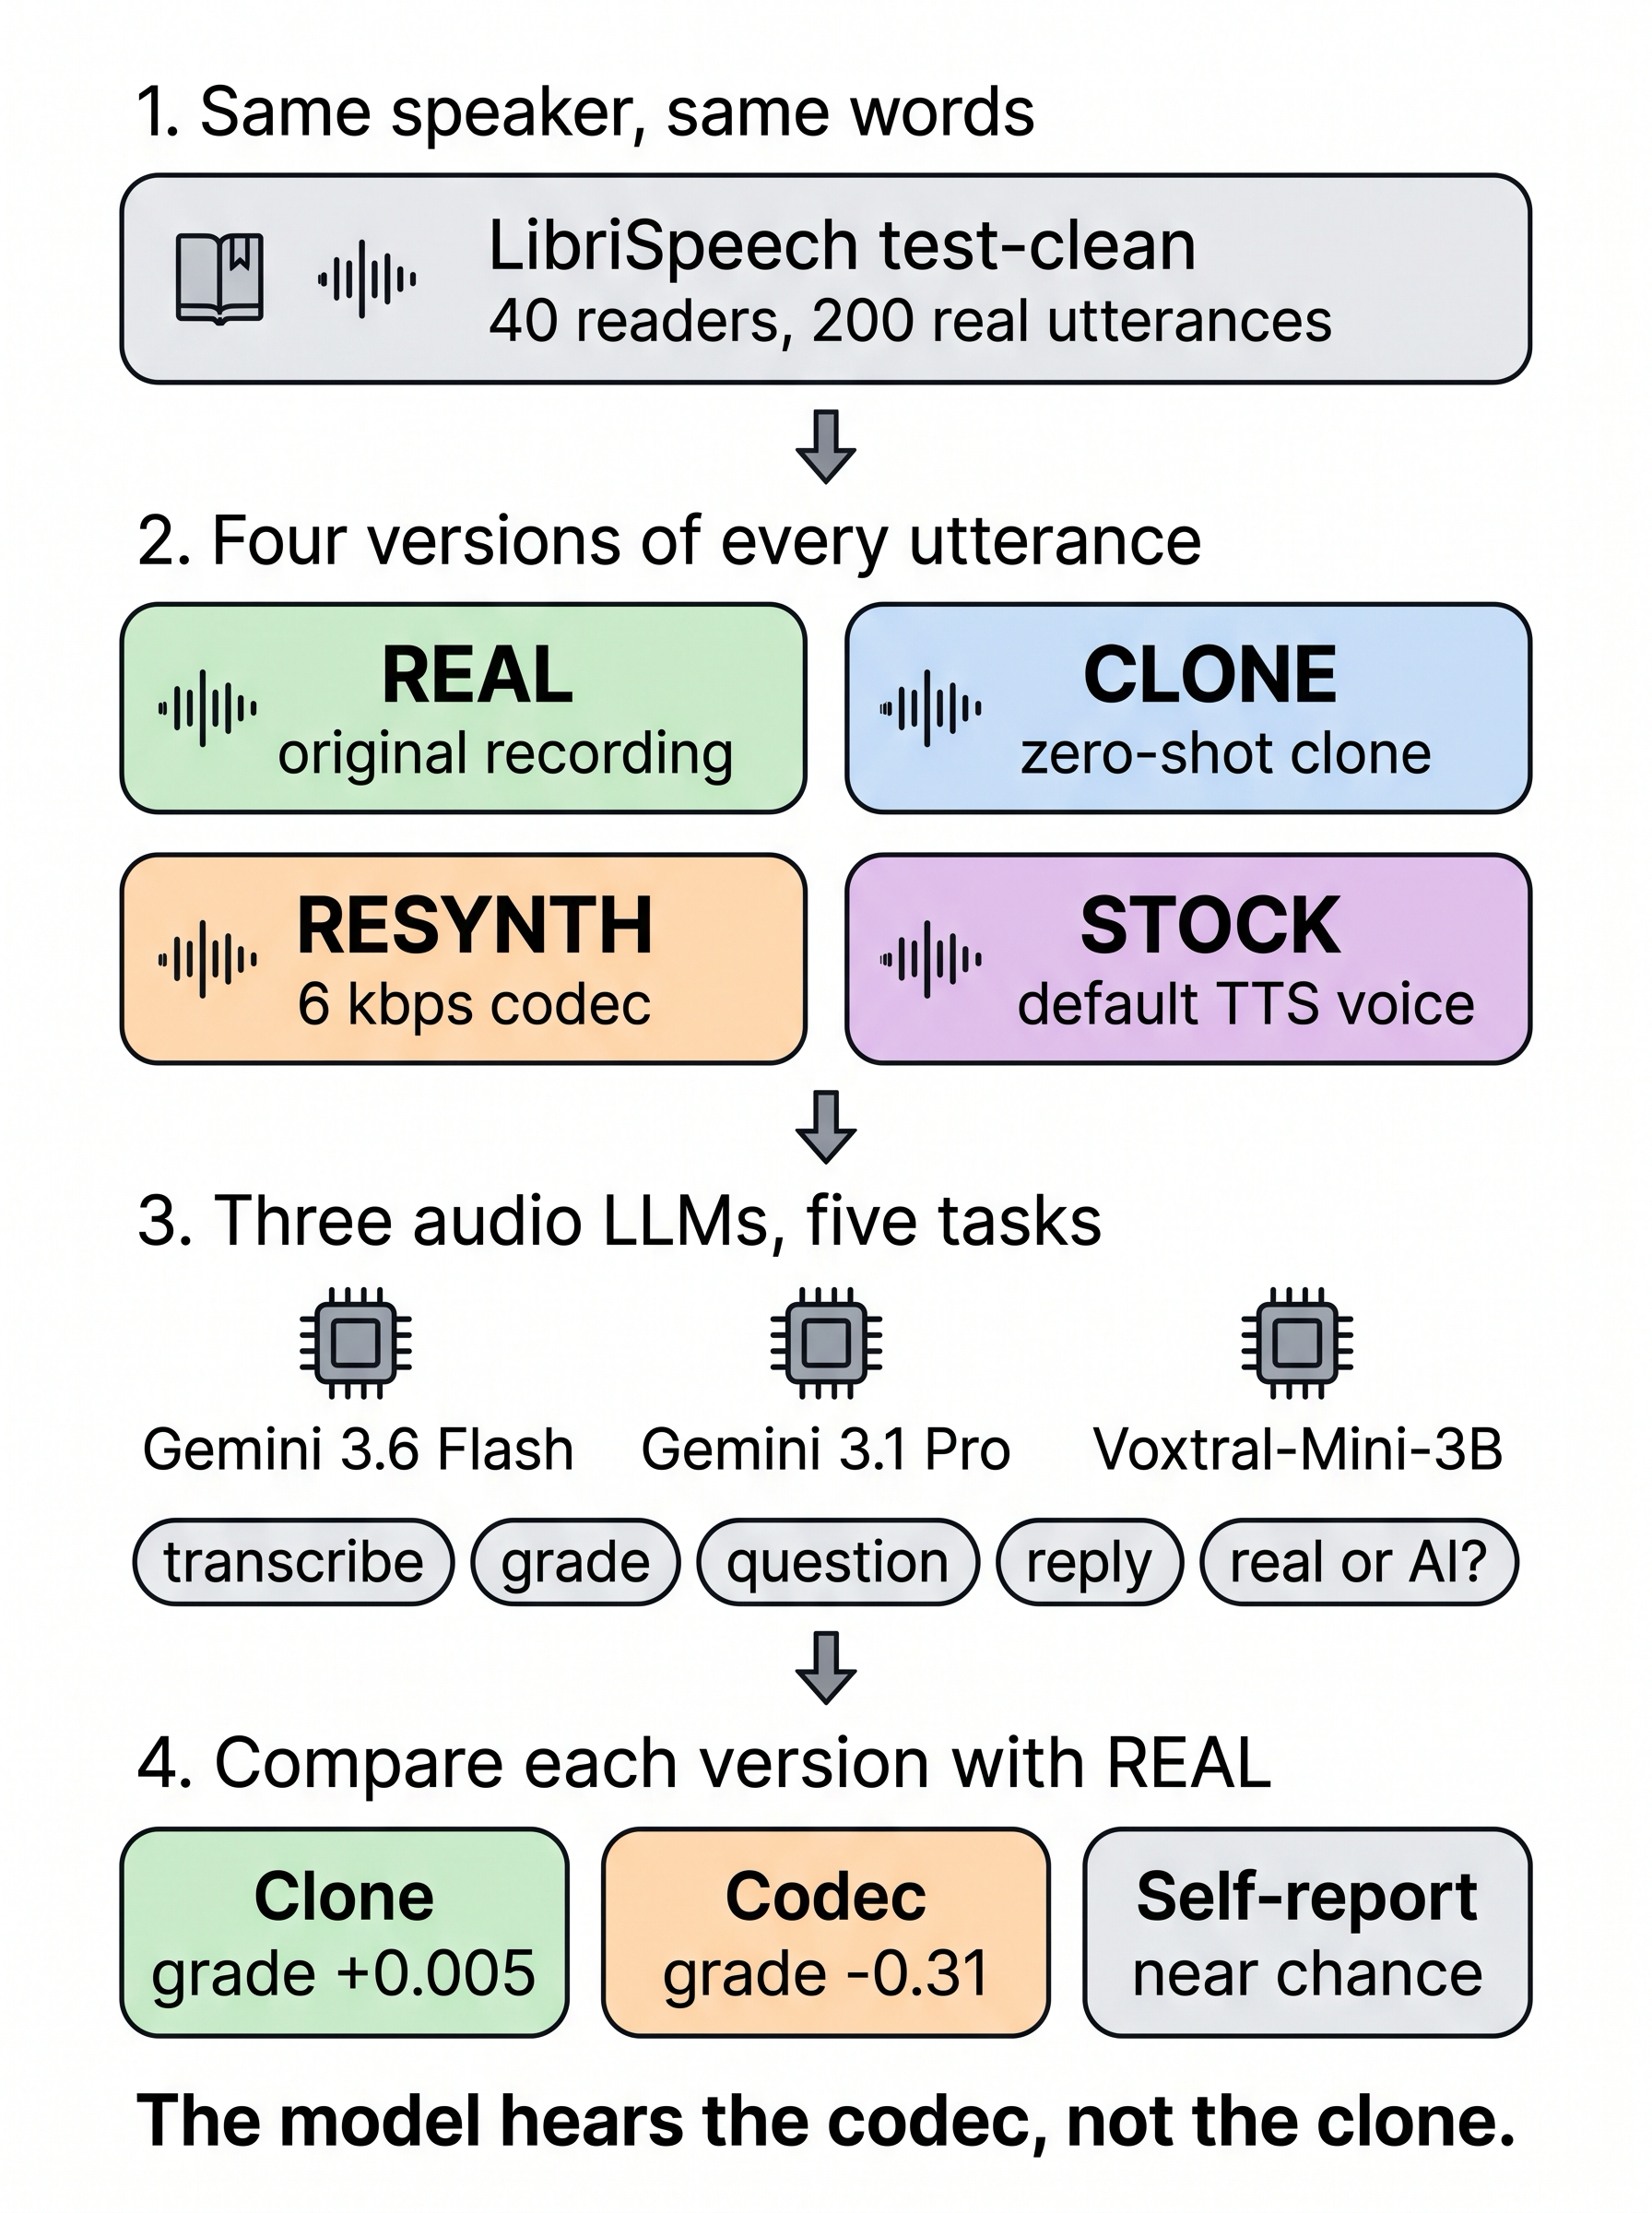
\includegraphics[width=\columnwidth]{assets/fig1_schematic.png}
\caption{Study design. (1) 200 real LibriSpeech utterances from 40 readers. (2) Each becomes four matched clips with the same words: the real recording, a same-speaker zero-shot clone, a 6 kbps codec re-encoding, and a stock TTS voice. (3) Three audio LLMs hear every clip and perform five tasks. (4) Each version is compared with REAL item by item. Schematic generated with Nano Banana 2 and checked by hand; numbers are from Table~\ref{tab:main}.}
\label{fig:schematic}
\end{figure}

\section{Related Work}
\label{sec:related}

\textbf{Synthetic stimuli in audio-model audits.} FairDialogue, BiasInEar, MedVoiceBias and The Voice Behind the Words generate their speaker variation with TTS or cloning and never evaluate real recordings \citep{a2510_02352,a2602_01030,a2511_06592,a2603_16941}. VIBE and RedVox build real-speech benchmarks in response to that practice \citep{a2604_17248,a2606_26968}, and HumDial-EIBench criticises TTS benchmarks without running the comparison \citep{a2604_11594}. Audio judges are robust to additive noise \citep{a2507_12705} but vulnerable to protocol shortcuts \citep{a2607_13477}, and ParaPairAudioBench uses same-transcript pairs to expose judge calibration failures \citep{a2606_24648}.

\textbf{What audio models know about synthetic speech.} Zero-shot detection by general audio models is at or below chance \citep{a2505_11079,a2512_10652,a2601_00777}, and the detectors that work are fine-tuned \citep{a2603_10725}. Human listeners reach about 80\% accuracy at spotting audio deepfakes after practice \citep{mueller2021} and increasingly mistake real speech for synthetic \citep{a2605_26136}. Hidden-state studies show that audio models encode cues they do not report \citep{a2605_13737,a2609_00727}, their uncertainty estimates do not transfer reliably across models and tasks \citep{a2604_25591}, and yes/no bias is a known failure mode \citep{a2604_19300}.

\textbf{Cloning, codecs and robustness.} Zero-shot cloners report speaker similarity at or near the ground-truth level on LibriSpeech test-clean with the reference protocol we use \citep{a2410_06885,a2412_10117,a2605_30748}. Neural codecs and their artifacts are the basis of codec-fake detection \citep{a2210_13438,a2501_08238}. Speech enhancement can make audio models worse \citep{a2601_10384}, in ways that standard quality metrics do not predict \citep{a2608_30348}, and encoder design changes how ASR degrades across speaker groups \citep{a2604_21276}. Synthetic voices are common in unsolicited calls \citep{a2609_11137}, listeners rate synthetic speech lower even when they cannot detect it \citep{a2605_28064}, and quality judgements vary widely across synthetic voices \citep{cambre2020}.

Table~\ref{tab:delineation} lists the closest studies and what each leaves open.

\begin{table*}[t]
\small
\centering
\resizebox{\textwidth}{!}{%
\begin{tabular}{>{\raggedright\arraybackslash}p{5.2cm}cccc}
\toprule
Study & Same speaker & Same words & Codec control & Behaviour + self-report \\
\midrule
Audio MultiChallenge \citep{a2512_14865} & -- & \checkmark & -- & -- \\
Counterfactual Audits \citep{a2608_06718} & -- & \checkmark & -- & -- \\
MedMosaic \citep{a2605_00969} & -- & -- & -- & -- \\
VoiceBench \citep{a2410_17196} & -- & \checkmark & -- & -- \\
BiasInEar \citep{a2602_01030} & clones only & \checkmark & -- & -- \\
ALLM4ADD, TriDF \citep{a2505_11079,a2512_10652} & -- & -- & -- & self-report only \\
PhonemeDF \citep{a2603_15037} & VC subset & \checkmark & -- & detector only \\
\midrule
\textbf{This work} & \checkmark & \checkmark & \checkmark & \checkmark \\
\bottomrule
\end{tabular}}
\caption{Closest prior studies. Only this work matches speaker and words, controls for codec artifacts, and measures behaviour and self-report on the same clips.}
\label{tab:delineation}
\end{table*}

\section{Experimental Setup}
\label{sec:setup}

\subsection{Dataset and matched stimuli}

\textbf{Speakers and items.} LibriSpeech test-clean \citep{librispeech} has 40 readers (20 women, 20 men) with gold transcripts. For each reader we draw, with a fixed seed, five target utterances of 4 to 12 seconds and 10 to 40 words, and one reference utterance of 5 to 10 seconds for cloning that does not overlap with the targets. This gives 200 items with a mean length of 7.6 seconds. Ten readers get a second reference clip for the clone-stability check.

\textbf{Four arms.} REAL is the original 16 kHz recording. CLONE is produced by Chatterbox \citep{chatterbox}, an open zero-shot cloning model, from the reader's reference clip and the target's gold transcript, with default settings and a fixed seed per item. RESYNTH is the real recording passed through EnCodec at 24 kHz and 6 kbps \citep{a2210_13438} and resampled to 16 kHz. It is still a real recording, with neural-codec artifacts added. STOCK is Chatterbox's built-in default voice reading the same transcript, so it is synthetic but not this speaker. All 850 clips (800 plus 50 second-reference clones) are normalised to $-23$ LUFS, padded with 0.2 s of silence, and frozen with a SHA-256 manifest before any model call. We disabled Chatterbox's watermarker so that CLONE and STOCK carry no signal that REAL and RESYNTH lack. Clone and stock clips are on average 0.8 s shorter than the real ones (6.7 s vs 7.6 s).

\subsection{Models and tasks}

Table~\ref{tab:models} lists the three models and how much of the grid each ran. The Gemini models were called through OpenRouter at temperature 0 with minimal reasoning, one clip per call, in random order. Voxtral-Mini-3B-2507 \citep{a2507_13264} ran locally in bfloat16 on CPU with greedy decoding, because its audio encoder crashed on the Apple GPU and no cloud GPU was available; at about 65 seconds per call we limited it to one item per reader. Other hosted audio model families were not available to us at the time.

\begin{table}[t]
\small
\centering
\begin{tabular}{lccl}
\toprule
Model & Arms & Items & Tasks \\
\midrule
Gemini 3.6 Flash (API) & 4 & 200 & O1--O5 \\
Gemini 3.1 Pro (API) & 4 & 60 & O2, O3, O4 \\
Voxtral-Mini-3B (local) & 2 & 40 & O2, O4 \\
\bottomrule
\end{tabular}
\caption{Models and coverage. Four arms = REAL, CLONE, RESYNTH, STOCK; two = REAL, CLONE. Pro ran 20 readers $\times$ 3 items; Voxtral 40 readers $\times$ 1 item.}
\label{tab:models}
\end{table}

Each clip is sent once per task with no conversation state. Verbatim prompts are in Appendix~\ref{app:prompts}.
\textbf{O1 Transcribe:} word error rate (WER) against the gold transcript after lowercasing and removing punctuation, $\mathrm{WER} = (S + D + I)/N$ for substitutions, deletions, insertions and reference length $N$ \citep{morris2004}.
\textbf{O2 Grade:} acting as an examiner, rate the clarity and fluency of the reading from 1 to 10 (integer).
\textbf{O3 Comprehend:} answer a four-option content question about the passage, generated once per item from the gold transcript by a text-only model.
\textbf{O4 Probe:} ``Is this audio a real human recording or AI-generated speech? Answer REAL or SYNTHETIC.''
\textbf{O5 Assist:} reply to the caller as a phone voice assistant in two or three sentences. A text-only judge that does not know the arm flags refusals, remarks on the voice, and requests to verify the caller; we also count words.

\subsection{Statistical analysis}

The unit of analysis is the item. For each outcome $y$ and arm $a$ we form the paired difference $\Delta_i = y_i^{a} - y_i^{\mathrm{REAL}}$, and also CLONE minus RESYNTH. Tests are two-sided sign-flip permutation tests that flip whole speakers (20,000 permutations; \citealp{good2005}). Intervals are 95\% percentile bootstrap intervals that resample speakers (10,000 resamples; \citealp{efron1979}). Effect sizes are the paired $d_z = \bar{\Delta}/s_{\Delta}$ \citep{lakens2013}. All 49 tests form one Benjamini-Hochberg family at $q \le 0.05$ \citep{bh1995}.

For the probe we report balanced accuracy, the mean of the rates at which real clips are called REAL and synthetic clips are called SYNTHETIC \citep{brodersen2010}. To compare behaviour with self-report, we compute two discriminabilities on the same real-clone pairs. The implicit one is $\mathrm{AUC}_{\text{grade}} = P(g^{\mathrm{REAL}} > g^{\mathrm{CLONE}}) + \tfrac12 P(g^{\mathrm{REAL}} = g^{\mathrm{CLONE}})$, the probability that the grade ranks the real clip above its clone \citep{hanley1982}; the explicit one is the same quantity computed from the probe answer. Chance is 0.5 for both. One script produces every number in the paper from the raw call logs.

\textbf{Pre-registration.} Five directions were recorded before any clip was cloned. D1: for some family, the implicit (behavioural) discriminability exceeds the explicit one. D2: the codec control explains less than half of the clone effect. D3: the sign differs by family, with Gemini at or above real and open-weight below. D4: explicit detection is below 60\% for every family. D5: WER does not differ between real and clone.

\textbf{Cost.} 6,420 hosted calls for \$2.99, plus about five hours of local compute for cloning and the open-weight model (Appendix~\ref{app:cost}).

\section{Results}
\label{sec:results}

Table~\ref{tab:main} reports every outcome by arm.

\begin{table*}[t]
\small
\centering
\resizebox{\textwidth}{!}{%
\begin{tabular}{llcccc}
\toprule
Model & Outcome & REAL & CLONE & RESYNTH & STOCK \\
\midrule
Gemini 3.6 Flash ($n{=}200$) & O2 grade (1--10) $\uparrow$ & \textbf{9.01} & \textbf{9.01} & 8.69$^\dagger$ & 9.00 \\
 & O1 word error rate $\downarrow$ & .029 & .027 & .031 & \textbf{.024} \\
 & O3 comprehension $\uparrow$ & .995 & .995 & .990 & \textbf{1.00} \\
 & O4 share called SYNTHETIC & .745 & .855 & .880 & .845 \\
 & O5 reply words & 30.5 & 30.7 & 30.8 & 31.2 \\
 & O5 refusal / voice remark & .015 / .015 & .010 / .050 & .015 / .025 & .005 / .020 \\
\midrule
Gemini 3.1 Pro ($n{=}60$) & O2 grade $\uparrow$ & 8.24 & \textbf{8.59} & 8.36 & \textbf{8.59} \\
 & O3 comprehension $\uparrow$ & \textbf{1.00} & \textbf{1.00} & \textbf{1.00} & \textbf{1.00} \\
 & O4 share called SYNTHETIC & .898 & .978 & .960 & .956 \\
\midrule
Voxtral-Mini-3B ($n{=}40$) & O2 grade $\uparrow$ & \textbf{8.48} & 8.30 & --- & --- \\
 & O4 share called SYNTHETIC & .000 & .000 & --- & --- \\
\bottomrule
\end{tabular}}
\caption{Every outcome by arm. Bold: best arm in each row where higher or lower is better. $^\dagger$: the paired difference against REAL survives Benjamini-Hochberg over all 49 tests. Paired differences with intervals are in Appendix~\ref{app:tables}.}
\label{tab:main}
\end{table*}

\subsection{The clone leaves behaviour unchanged}
\label{sec:results-clone}

Gemini 3.6 Flash grades both the real recordings and the clones at 9.01 on average. The paired difference is $+0.005$ points (95\% interval $-0.155$ to $+0.161$, $p = 1.0$, $d_z = 0.00$, $n = 200$). The stock voice is graded 8.995, a difference of $-0.005$ ($p = 1.0$). Neither a synthetic voice in general nor a clone of this reader moves the grade (Figure~\ref{fig:grade}). WER is 2.9\% on real, 2.7\% on clone ($p = 0.87$) and 2.4\% on stock. Content questions are answered correctly on 99.5\% of real and clone clips, which only tells us that the clones are fully intelligible. Assistant replies have the same length (30.5 vs 30.7 words) and refusal rate (1.5\% vs 1.0\%), and none asks the caller to prove they are human. The judge flagged a remark about the voice in 1.5\% of real and 5\% of clone replies. We read 24 of these replies by hand, and every flag was the model noting that the caller seemed to be reading from a book, not a remark about the voice (Appendix~\ref{app:audit}).

Gemini 3.1 Pro, on 60 items, grades real at 8.24 and clone at 8.59, a difference of $+0.35$ (interval $-0.90$ to $+1.46$, $p = 0.60$). It answers every content question correctly on every arm. The interval is wide because Pro's grades vary more between repeated calls than Flash's; it includes both zero and the Flash estimate.

\begin{figure*}[t]
\centering
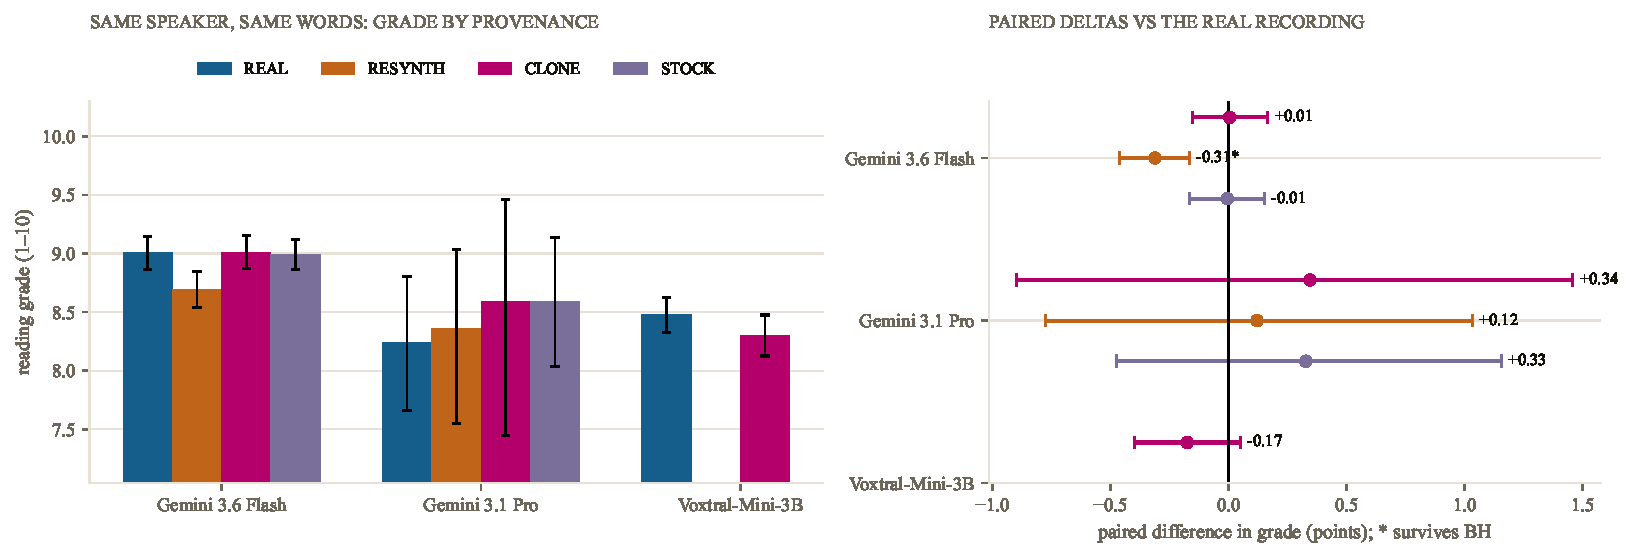
\includegraphics[width=0.82\textwidth]{assets/fig2_grade.pdf}
\caption{\textbf{Left:} reading grade by arm and model, with 95\% speaker-bootstrap intervals. \textbf{Right:} paired differences against the real recording; a star marks a difference that survives correction. The clone and the stock voice sit on zero, while the codec re-encoding is graded lower.}
\label{fig:grade}
\end{figure*}

\subsection{The codec lowers the grade}
\label{sec:results-codec}

RESYNTH is the same real waveform after a 6 kbps codec round trip. Flash grades it 8.69, which is $-0.312$ points against real (interval $-0.460$ to $-0.162$, $p = 3.5\times10^{-4}$, $d_z = -0.25$) and $-0.320$ against the clone ($p = 4.5\times10^{-4}$). These are the only two of the 49 tests that survive correction. WER on RESYNTH is 3.1\% ($p = 0.86$ against real) and comprehension is 99\%, so the codec lowers the grade without making the speech harder to understand.

The result is also a positive control: with 200 paired items the design detects a third-of-a-point shift, so the null result for the clone is not caused by low power. It reverses pre-registered direction D2, which assumed there would be a clone effect for the codec to partly explain. There is no clone effect, and the codec has an effect of its own. The model reacts to something in the signal that a 6 kbps codec introduces and a current zero-shot clone does not. On Pro the RESYNTH difference is $+0.12$ ($p = 0.81$, $n = 60$), so we cannot tell whether the codec effect is specific to Flash or too small for Pro's sample size.

\subsection{Asked directly, the models cannot tell and lean towards ``synthetic''}
\label{sec:results-probe}

Flash calls 74.5\% of real recordings synthetic, and 85.5\% of clones, 88.0\% of codec re-encodings and 84.5\% of stock clips (Figure~\ref{fig:probe}, left). Pro calls 89.8\% of real recordings and 97.8\% of clones synthetic. The clone raises Flash's synthetic share by 11.0 points (interval 3.0 to 19.0, $p = 0.015$) and the codec by 13.5 points ($p = 0.0085$). Neither survives correction, and the two do not differ from each other ($p = 0.48$). The answer reacts to re-encoding at least as much as to cloning, and it is dominated by a prior that speech is synthetic.

Table~\ref{tab:disc} compares behaviour with self-report on the same real-clone pairs. On Flash the grade-based AUC is 0.503, which is chance, against 0.555 for the stated answer (difference $-0.05$, interval $-0.08$ to $+0.02$). On Pro both are 0.53. The comprehension-based AUC is 0.50 on both Gemini models. D1 is not supported for Gemini: the models do not discriminate in their behaviour any better than in their answers.

\begin{table}[t]
\small
\centering
\setlength{\tabcolsep}{4pt}
\begin{tabular}{lcccc}
\toprule
 & \multicolumn{2}{c}{Balanced acc.} & \multicolumn{2}{c}{AUC, real vs clone} \\
\cmidrule(lr){2-3}\cmidrule(lr){4-5}
Model & vs clone & vs stock & grade & answer \\
\midrule
Gemini Flash & \textbf{0.555} & \textbf{0.55} & 0.503 & \textbf{0.555} \\
Gemini Pro & 0.54 & --- & 0.53 & 0.53 \\
Voxtral & 0.50 & --- & \textbf{0.575} & 0.50 \\
\bottomrule
\end{tabular}
\caption{Provenance discriminability; chance is 0.5 everywhere. ``Grade'' is the implicit signal (the model's own grade), ``answer'' the explicit one (the probe). Bold: best model per column. No value exceeds 0.58.}
\label{tab:disc}
\end{table}

\begin{figure*}[t]
\centering
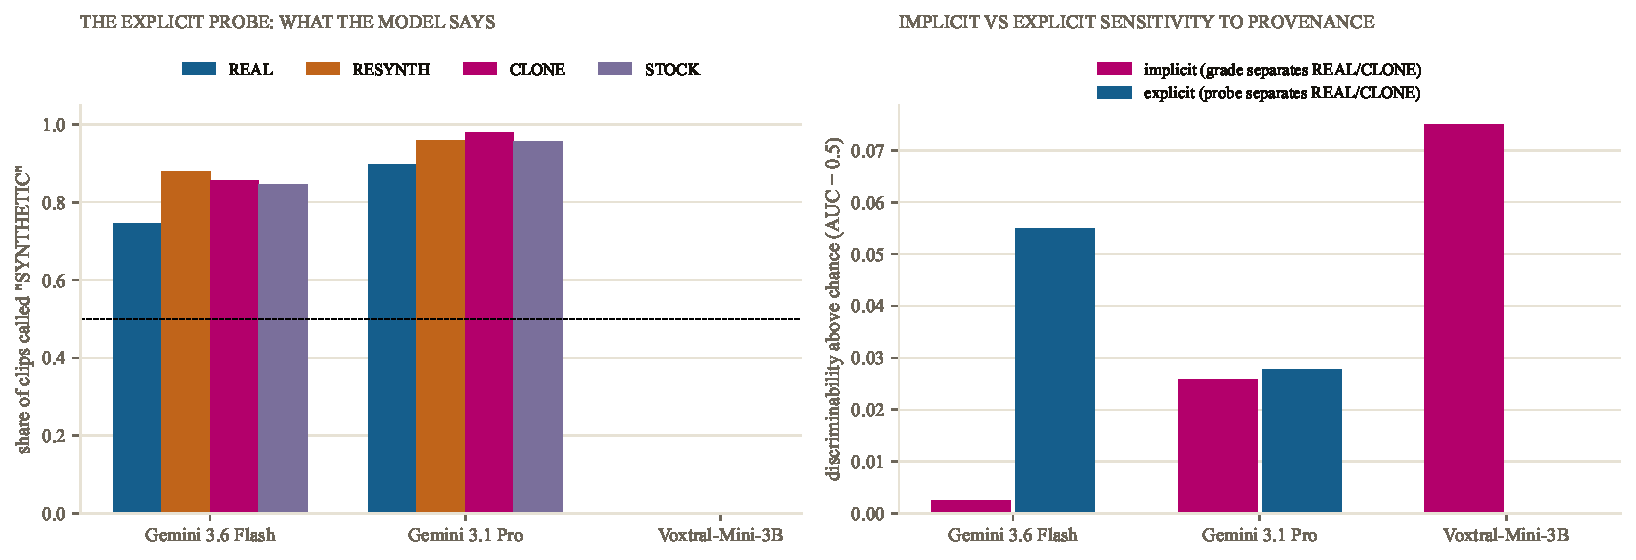
\includegraphics[width=0.82\textwidth]{assets/fig3_probe.pdf}
\caption{\textbf{Left:} share of clips called SYNTHETIC, by arm. Most real recordings are called synthetic. \textbf{Right:} how far each model separates real from clone above chance, from its own grades (implicit) and from its stated answer (explicit). Both are close to zero, and the implicit signal is not larger.}
\label{fig:probe}
\end{figure*}

\subsection{The open-weight model leans the other way}
\label{sec:results-open}

Voxtral-Mini-3B grades the real recordings 8.48 and the clones 8.30 on its 40-item subset. The paired difference is $-0.175$ (interval $-0.40$ to $+0.05$, $p = 0.19$, $d_z = -0.25$). This is the direction MedMosaic reported for open-weight models and the one we pre-registered in D3, but it is small and the interval includes zero. Voxtral answers REAL for all 79 parsed clips, real and clone alike, which is the opposite of Gemini's bias. Its grades separate real from clone at AUC 0.575 against 0.50 for its answer (difference $+0.075$, interval $0.00$ to $+0.175$). This is the only place in the study where the D1 pattern appears, and because the lower bound of the interval is zero we treat it as suggestive. The differences between families in the clone effect (Flash minus Voxtral $+0.18$, $p = 0.45$; Pro minus Voxtral $+0.65$, $p = 0.44$) are not significant at these sample sizes.

\subsection{Comparison with earlier synthetic-versus-real reports}
\label{sec:results-baselines}

Table~\ref{tab:baselines} places our estimates next to the published comparisons that motivated this study. The earlier studies compare synthetic and real arms with different speakers and recording conditions, and they report gaps in both directions, some of more than 12 points. When speaker and words are matched, the Gemini gap disappears. The one effect we do find comes from compression, which was not controlled in the earlier comparisons. This suggests that part of what they measured was a difference in recording and encoding conditions rather than in provenance. For explicit detection our numbers agree with earlier zero-shot results, which were also at or below chance.

\begin{table*}[t]
\small
\centering
\begin{tabular}{>{\raggedright\arraybackslash}p{3.1cm}>{\raggedright\arraybackslash}p{2.6cm}>{\raggedright\arraybackslash}p{2.3cm}>{\raggedright\arraybackslash}p{4.2cm}}
\toprule
Study & Design & Models & Synthetic minus real \\
\midrule
Audio MultiChallenge \citep{a2512_14865} & stock TTS vs human, different voice & various & $+7.5\%$ (text output), $-2.5\%$ (audio output) \\
MedMosaic \citep{a2605_00969} & unmatched subsets & Gemini; open-weight & $+1.4$ to $+3.3$; mostly negative, four below $-12$ \\
VoiceBench \citep{a2410_17196} & same questions, TTS vs crowd-recorded & various & all models better on synthetic \\
\midrule
\textbf{Ours, clone} & matched speaker, words & Gemini 3.6 Flash & $\mathbf{+0.005}$ grade [$-0.16$, $+0.16$] \\
\textbf{Ours, clone} & matched speaker, words & Voxtral-Mini-3B & $-0.18$ grade [$-0.40$, $+0.05$] \\
\textbf{Ours, codec} & same recording & Gemini 3.6 Flash & $-0.31$ grade [$-0.46$, $-0.16$]$^\dagger$ \\
\midrule
ALLM4ADD / TriDF \citep{a2505_11079,a2512_10652} & zero-shot detection & Qwen-Audio; Gemini 2.5 Pro & at or below chance \\
\textbf{Ours, probe} & matched pairs & Flash / Pro / Voxtral & bal.\ acc.\ \textbf{0.555} / 0.54 / 0.50 \\
\bottomrule
\end{tabular}
\caption{Our matched estimates next to earlier reports. Earlier numbers are copied from each paper and use their own metrics (accuracy or score points); ours are on the 10-point grade with 95\% intervals. Bold: the estimate closest to zero gap, and the highest detection accuracy. $^\dagger$ survives correction.}
\label{tab:baselines}
\end{table*}

\subsection{Noise floor, clone stability, and pre-registered directions}
\label{sec:results-batteries}

\textbf{Noise floor.} We re-ran 30 items five times each on Flash at temperature 0. The grade changed across the five identical calls in 83\% of cells (mean within-cell standard deviation 0.57 points), and the probe answer changed in 37\%. The clone effect ($+0.005$) is far inside this floor, which is expected: the $\pm 0.16$ interval is the precision of a 200-item average, not of a single call. The codec effect ($-0.31$) is about half of one call's standard deviation and is detected through pairing.

\textbf{Clone stability.} For ten readers we cloned every target twice from two different reference clips. The two clones' grades differ by 0.64 points on average (signed mean $-0.28$), and the probe answer differs on 38\% of items. Variation between two clones of the same speaker is about the size of the codec effect and four times the clone-versus-real difference, so an audit that uses one clone per speaker carries this much sampling noise.

\textbf{Pre-registered directions.} D1 (implicit exceeds explicit): not supported on either Gemini model; suggestive on Voxtral. D2 (codec explains under half of the clone effect): reversed, since there is no clone effect and the codec effect is the only one present. D3 (sign differs by family): visible in the point estimates (Gemini at or above real, Voxtral below) but not significant. D4 (explicit detection under 60\%): holds for all three models. D5 (equal WER): holds, 2.7\% vs 2.9\%, $p = 0.87$.

\section{Discussion}
\label{sec:discussion}

\textbf{For audit designers.} For the Gemini models, using synthetic voices in place of real ones is supported to within about a sixth of a grade point: a clone produces the same grades, transcripts, comprehension and assistant replies as the real recording. The codec result adds a condition. If the synthetic arm of an audit is compressed differently from the real arm, the audit will measure the compression and not the voice. Both arms should go through the same encoding chain. Audits should also use more than one clone per speaker, since clone-to-clone variation is as large as the codec effect.

\textbf{For deployments.} A clone of a person is treated the same as that person, so a voice-banking user or a TTS user is not penalised for using a synthetic voice. However, a model's own answer to ``is this a real person'' is not usable. Flash calls three out of four real callers synthetic and Voxtral calls every caller real. A system that relies on that answer to make a decision would reject most real callers with Gemini and accept every clone with Voxtral.

\section{Conclusion}

We held the speaker and the words fixed and asked whether audio language models treat a voice clone differently from the real recording. Gemini 3.6 Flash does not, to within a sixth of a grade point over 200 paired items, with the same transcription, comprehension and assistant behaviour. Gemini 3.1 Pro agrees within a wider interval, and Voxtral-Mini-3B leans slightly the other way without reaching significance. All three models react more to a 6 kbps codec than to the clone, and none can say reliably whether a voice is real. Synthetic stimuli are a valid tool for auditing these models as long as compression is equalised across arms, and a model's own judgement about whether a speaker is real should not be used in deployment.

\textbf{Future work.} Four extensions follow directly. First, run the full grid on an open-weight model with a GPU, and on more hosted families, to test whether the sign difference in D3 is real. Second, use harder grading tasks with lower baseline scores, and request-style content recorded by real speakers, so that the grade and the assistant task have room to move. Third, vary the codec bitrate and the synthesiser quality to locate the point where the models start to react. Fourth, look inside an open-weight model's hidden states for provenance information that neither its grades nor its answers show.

\section*{Limitations}

Our clones are high quality: WER matches the real recordings and comprehension is at ceiling. The results apply to good zero-shot clones, not to synthetic speech in general. A weaker synthesiser would probably fall between CLONE and RESYNTH, and the codec result suggests the models would react to it. LibriSpeech readers may appear in TTS training data, so the cloner may have seen these speakers. That would make the clones better, which strengthens the null result for behaviour but limits what we can say about unseen speakers.

The passages are audiobook sentences, so the assistant task (O5) asks the model to reply to a caller who is reading a book aloud. The replies mostly ask what the caller wants, which may be why O5 shows no difference. Comprehension is at ceiling on every arm and serves only as an intelligibility check. The grade is also close to its ceiling (about 9.0 for Flash), which leaves little room for a penalty. Two observations limit this concern: the codec penalty is visible in the same range, and Pro, whose grades are lower (8.2 to 8.6), shows no clone penalty either.

Grades are noisy: 83\% of cells change across identical calls at temperature 0. Our paired averages are precise to about a sixth of a point over 200 items, and every claim is limited to that precision. Pro ran 60 items and Voxtral 40 items on two tasks, so their intervals are much wider. The probe uses a single wording, and the strong synthetic bias may partly come from that wording.

\section*{Ethical Considerations}
Voices are cloned only from LibriSpeech, a public-domain audiobook corpus released under CC BY 4.0. The clones are used only as matched stimuli and are not released as voices. No deployed system was tested beyond public model APIs. We disabled the clone generator's watermark so that the clone arm carries no signal the real arm lacks; the clips exist only for this measurement and can be regenerated only from public data and our scripts. Our finding that models cannot detect clones should not be read as support for using clones to deceive; it is a warning against relying on audio models to detect them.

\paragraph{Reproducibility.}
The item list, the clone, resynthesis and freeze scripts with the corpus hash, every prompt, every runner, the raw call logs, the single analysis script that produces every number in this paper, the audited samples and the spend log accompany this submission. All audio can be regenerated from LibriSpeech with the scripts.

\section*{Use of AI Assistants}
\textbf{In the experiments:} Gemini 3.6 Flash, Gemini 3.1 Pro and Voxtral-Mini-3B are the subjects of the study. Gemini 3.6 Flash, in text-only mode, also generated the O3 comprehension questions and served as the blind O5 judge. Chatterbox generated the CLONE and STOCK audio. \textbf{Experimental setup and code:} an AI coding assistant (Claude) helped write the data-preparation, inference and analysis scripts; every script was run and its outputs checked by the author. \textbf{Figures:} Figure~\ref{fig:schematic} was generated with Nano Banana 2 (Gemini 3.1 Flash Image) from a written description of the pipeline, and every label was checked by hand against the paper; the data figures were drawn with matplotlib from the analysis output. \textbf{Writing:} Claude helped draft and edit the text; the author revised every section by hand. All design choices, statistical decisions and claims are the author's, and every reported number was checked against the scripted analysis output.
